\documentclass[11pt,a4paper]{article}
\usepackage[utf8]{inputenc}
\usepackage[T1]{fontenc}
\usepackage{geometry}
\usepackage{graphicx}
\usepackage{listings}
\usepackage{xcolor}
\usepackage{hyperref}
\usepackage{float}
\usepackage{enumitem}
\usepackage{booktabs}
\usepackage{fancyhdr}
\usepackage{titlesec}
\usepackage{tcolorbox}
\usepackage{parskip}
\usepackage{caption}
\usepackage{tikz}
\usetikzlibrary{arrows.meta,positioning}

\geometry{margin=2.5cm}

\hypersetup{
    colorlinks=true,
    linkcolor=blue!70!black,
    urlcolor=blue!60!black,
    citecolor=blue!70!black
}

\definecolor{codebg}{RGB}{245,245,245}
\definecolor{codeframe}{RGB}{200,200,200}
\definecolor{codegreen}{RGB}{40,160,40}
\definecolor{codepurple}{RGB}{130,80,180}
\definecolor{codegray}{RGB}{100,100,100}
\definecolor{graphblue}{RGB}{220,235,255}
\definecolor{graphpurple}{RGB}{238,228,255}
\definecolor{graphorange}{RGB}{255,234,204}
\definecolor{graphgreen}{RGB}{38,150,78}
\definecolor{graphred}{RGB}{196,53,53}

\lstdefinestyle{codestyle}{
    backgroundcolor=\color{codebg},
    frame=single,
    rulecolor=\color{codeframe},
    basicstyle=\ttfamily\small,
    breaklines=true,
    columns=fullflexible,
    keepspaces=true,
    showstringspaces=false,
    xleftmargin=0.5cm,
    xrightmargin=0.5cm,
    aboveskip=0.5em,
    belowskip=0.5em,
    commentstyle=\color{codegray},
    keywordstyle=\color{codepurple},
    stringstyle=\color{codegreen},
}

\newtcolorbox{rationale}{
    colback=blue!5!white,
    colframe=blue!40!black,
    title=Design Rationale,
    fonttitle=\bfseries,
    boxrule=0.5pt,
    arc=2mm,
}

\newtcolorbox{designnote}{
    colback=yellow!8!white,
    colframe=orange!60!black,
    title=Key Insight,
    fonttitle=\bfseries,
    boxrule=0.5pt,
    arc=2mm,
}

\newtcolorbox{successbox}[1]{
    colback=green!5!white,
    colframe=green!40!black,
    title=#1,
    fonttitle=\bfseries,
    boxrule=0.5pt,
    arc=2mm,
}

\newtcolorbox{reflectionbox}{
    colback=purple!5!white,
    colframe=purple!40!black,
    title=Reflection,
    fonttitle=\bfseries,
    boxrule=0.5pt,
    arc=2mm,
}

\tikzset{
    graphbase/.style={
        rectangle,
        rounded corners=2mm,
        draw=black!60,
        thick,
        minimum width=2.8cm,
        minimum height=0.95cm,
        align=center,
        font=\small
    },
    datanode/.style={graphbase, fill=graphblue},
    llmnode/.style={graphbase, fill=graphpurple},
    evalnode/.style={graphbase, fill=graphorange},
    hybridnode/.style={graphbase, fill=graphblue, draw=codepurple, line width=1pt},
    archbox/.style={graphbase, fill=blue!8!white, minimum width=3.2cm, minimum height=1.1cm},
    mergepoint/.style={circle, fill=graphgreen, draw=graphgreen, minimum size=3.5pt, inner sep=0pt},
    line/.style={-Latex, thick, draw=black!70},
    successline/.style={-Latex, ultra thick, draw=graphgreen},
    retryline/.style={-Latex, ultra thick, draw=graphred},
}

\pagestyle{fancy}
\fancyhf{}
\fancyhead[L]{\small Seismic Command --- LangGraph Integration}
\fancyhead[R]{\small Yunus Emre Balci}
\fancyfoot[C]{\thepage}

\title{\textbf{LangGraph Integration in Seismic Command:\\[0.3em]
Stateful Graph-Based AI Orchestration\\
for Earthquake Risk Analysis}}
\author{Yunus Emre Balci \\ Akdeniz University --- Computer Engineering}
\date{April 19, 2026 \\[0.3em]
\small Stack: LangGraph 0.2 + LangSmith + Groq (LLaMA-3.3-70B) + FastAPI + Angular}

\begin{document}

\maketitle
\thispagestyle{fancy}

\tableofcontents
\newpage

% ============================================================
\section{Introduction}
% ============================================================

\textbf{Seismic Command} is a full-stack earthquake safety platform for Turkey, built with an Angular frontend, a Spring Boot backend, and a Python-based AI layer. This report documents the \textbf{LangGraph integration} added to the existing project---which already contained a CrewAI multi-agent pipeline---demonstrating that both frameworks coexist and run concurrently within the same codebase.

LangGraph was chosen specifically for its ability to model \textit{stateful, conditional workflows} as directed graphs. Unlike a simple chain of LLM calls, LangGraph allows branching, feedback loops, and parallel fan-out, which are exactly the patterns required for dynamic earthquake risk assessment.

\begin{rationale}
The LangGraph layer exposes \textbf{two primary user-facing graphs}:
\begin{itemize}[leftmargin=1.2em]
    \item \textbf{Chat Graph} --- A stateful multi-turn conversational assistant that classifies user intent and routes to the appropriate data-fetching or answering pipeline.
    \item \textbf{Building Risk Graph} --- An agentic evaluation loop that scores a building's earthquake risk and uses an LLM evaluator to refine its own output before returning a final result.
\end{itemize}
Both graphs run as async FastAPI endpoints on port 8002 and are consumed by the same existing Spring Boot + Angular application that already integrates CrewAI.
\end{rationale}

\begin{designnote}
This submission focuses on the two LangGraph workflows that are already surfaced in the product UI and easiest to discuss in class: \texttt{/graph/chat} and \texttt{/graph/building-risk}. The repository may contain additional experimental graph modules, but they are outside the core scope of this report.
\end{designnote}

\noindent\textbf{Git repository:} \url{https://github.com/YunusEmre3757/advenced_web}

% ============================================================
\section{Purpose of LangGraph in This Project}
% ============================================================

LangGraph solves three specific problems that a plain LLM call cannot:

\begin{enumerate}[leftmargin=1.5em]
    \item \textbf{Intent routing at runtime.} A user's question about ``last week's earthquakes'' requires a different pipeline than a question about ``is my building safe.'' LangGraph's conditional edges make this routing explicit and inspectable.

    \item \textbf{Multi-turn memory.} The Chat Graph uses LangGraph's built-in \texttt{add\_messages} reducer with a PostgreSQL checkpointer, so conversation history persists across HTTP requests without any manual state management.

    \item \textbf{Agentic self-correction.} The Building Risk Graph implements an evaluator-worker feedback loop: if the LLM-generated risk summary is too short or misses key factors, the evaluator node injects feedback and the graph re-enters the analysis branch (up to 2 retries). This pattern cannot be expressed as a simple chain.
\end{enumerate}

% ============================================================
\section{System Architecture}
% ============================================================

The overall system has three layers. The Angular frontend communicates with the Spring Boot backend (Java), which in turn calls the LangGraph service (Python/FastAPI) for AI-intensive operations.

\begin{figure}[H]
\centering
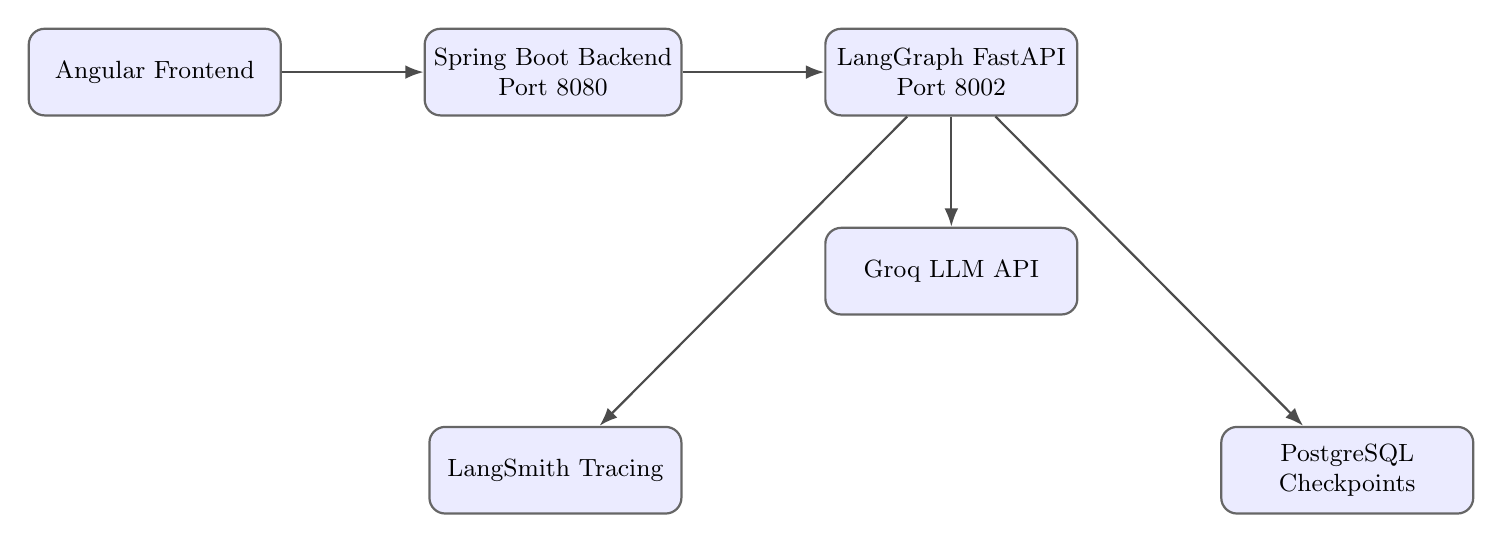
\begin{tikzpicture}[node distance=1.4cm and 1.8cm]
    \node[archbox] (frontend) {Angular Frontend};
    \node[archbox, right=of frontend] (backend) {Spring Boot Backend\\Port 8080};
    \node[archbox, right=of backend] (graphsvc) {LangGraph FastAPI\\Port 8002};

    \node[archbox, below=of graphsvc] (groq) {Groq LLM API};
    \node[archbox, below left=of groq] (langsmith) {LangSmith Tracing};
    \node[archbox, below right=of groq] (postgres) {PostgreSQL\\Checkpoints};

    \draw[line] (frontend) -- (backend);
    \draw[line] (backend) -- (graphsvc);
    \draw[line] (graphsvc) -- (groq);
    \draw[line] (graphsvc) -- (langsmith);
    \draw[line] (graphsvc) -- (postgres);
\end{tikzpicture}
    \caption{High-level system architecture for the LangGraph integration. The frontend calls Spring Boot, which proxies AI-intensive requests to the LangGraph service.}
    \label{fig:architecture}
\end{figure}

\subsection{Technology Stack}

\begin{table}[H]
\centering
\begin{tabular}{@{}lll@{}}
\toprule
\textbf{Component} & \textbf{Technology} & \textbf{Purpose} \\
\midrule
LLM provider       & Groq --- LLaMA-3.3-70B-Versatile & Graph node LLM calls \\
Graph framework    & LangGraph 0.2                    & Stateful graph orchestration \\
Tracing            & LangSmith 0.3                    & Run monitoring and debugging \\
Structured output  & Pydantic v2                      & Typed LLM responses \\
API layer          & FastAPI + uvicorn                & Async HTTP endpoints \\
Persistence        & PostgreSQL + langgraph-checkpoint & Multi-turn chat memory \\
Frontend           & Angular 18                       & User interface \\
Backend            & Spring Boot 3                    & Data layer and routing \\
Co-existing agent  & CrewAI                           & Parallel multi-agent tasks \\
\bottomrule
\end{tabular}
\caption{Technology stack used in the LangGraph integration.}
\end{table}

\subsection{LangGraph Service Entry Point}

The service starts with a FastAPI lifespan that initialises LangSmith tracing and the PostgreSQL checkpointer before any request is served:

\begin{lstlisting}[style=codestyle, language=Python]
@asynccontextmanager
async def lifespan(_app: FastAPI):
    if LANGSMITH_TRACING:
        os.environ.setdefault("LANGCHAIN_TRACING_V2", "true")
        os.environ.setdefault("LANGCHAIN_PROJECT", LANGSMITH_PROJECT)

    checkpointer = await setup_checkpointer()
    reset_chat_graph()
    get_chat_graph(checkpointer)   # compile once, reuse across requests
    yield
    await get_spring_client().close()
    await close_checkpointer()
\end{lstlisting}

% ============================================================
\section{Graph 1: Chat Graph}
% ============================================================

\subsection{Purpose and Topology}

The Chat Graph is a stateful multi-turn assistant. It answers earthquake-related questions in Turkish, using Kandilli Observatory data fetched live from the Spring Boot backend.

\begin{figure}[H]
\centering
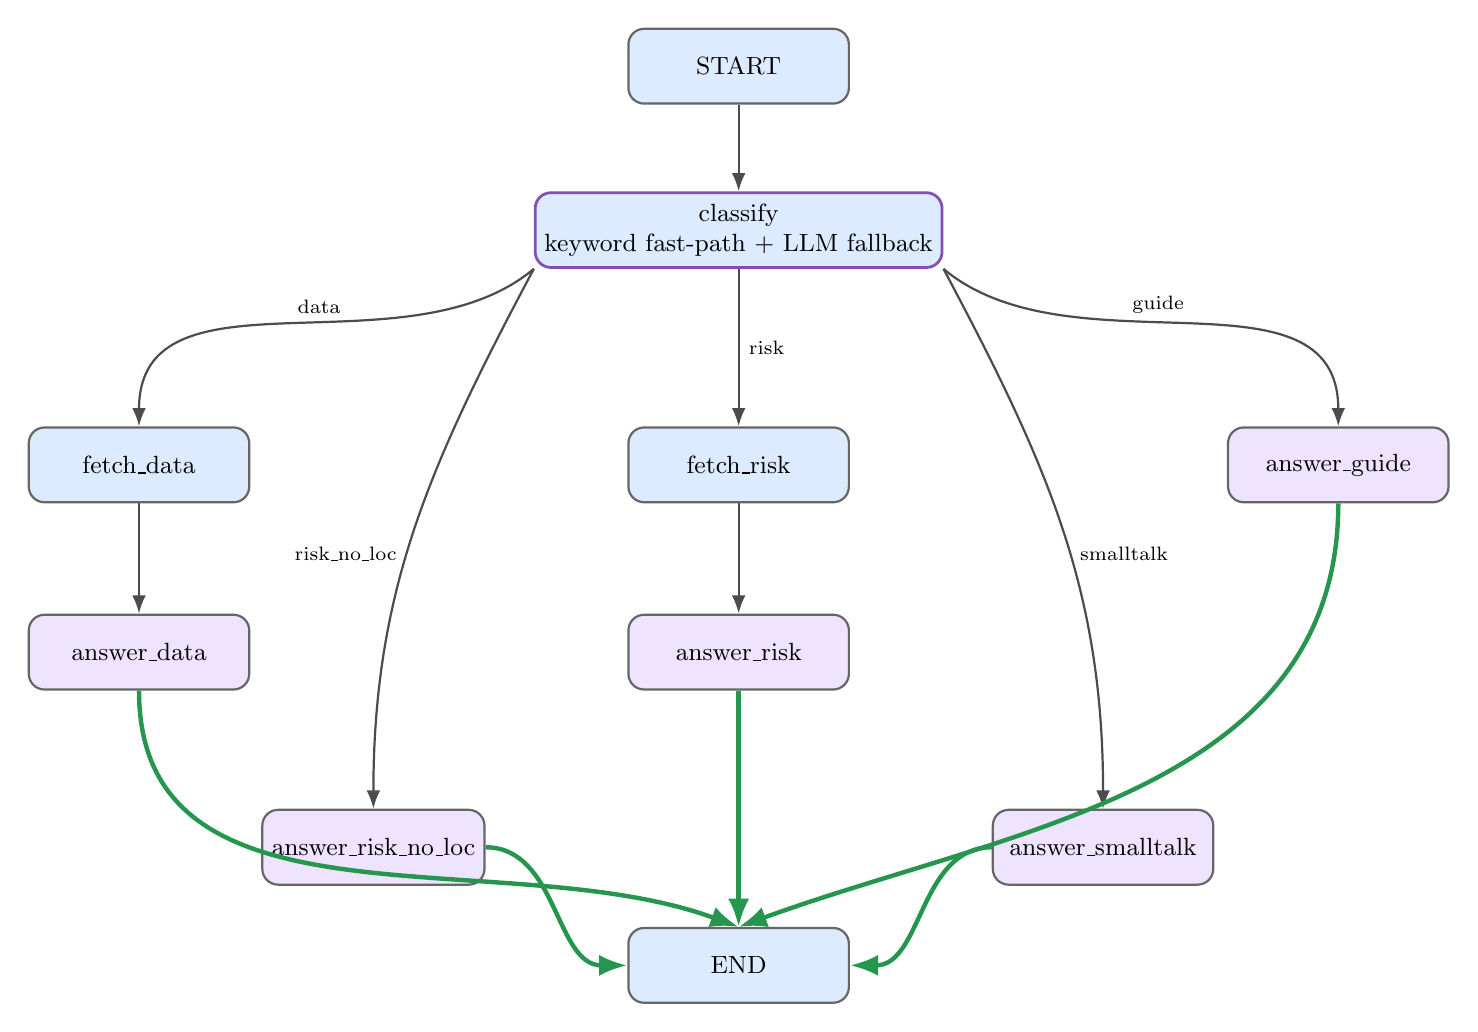
\begin{tikzpicture}[font=\small, node distance=1.0cm and 1.6cm]
    % Core flow
    \node[datanode] (start) {START};
    \node[hybridnode, below=1.1cm of start, minimum width=4.4cm] (classify) {classify\\keyword fast-path + LLM fallback};

    % Route targets from classify
    \node[datanode, below left=2.0cm and 3.6cm of classify] (fetchdata) {fetch\_data};
    \node[datanode, below=2.0cm of classify] (fetchrisk) {fetch\_risk};
    \node[llmnode, below right=2.0cm and 3.6cm of classify] (answerguide) {answer\_guide};

    % Downstream answer nodes
    \node[llmnode, below=1.4cm of fetchdata] (answerdata) {answer\_data};
    \node[llmnode, below=1.4cm of fetchrisk] (answerrisk) {answer\_risk};
    \node[llmnode, below left=1.5cm and 1.8cm of answerrisk] (answernoloc) {answer\_risk\_no\_loc};
    \node[llmnode, below right=1.5cm and 1.8cm of answerrisk] (answersmall) {answer\_smalltalk};

    \node[datanode, below=3.0cm of answerrisk] (end) {END};

    % Entry
    \draw[line] (start) -- (classify);

    % Conditional routes from classify (matches _route mapping)
    \draw[line] (classify.south west) to[out=220,in=90] node[pos=0.44, above, font=\scriptsize] {data} (fetchdata.north);
    \draw[line] (classify.south) -- node[right, font=\scriptsize] {risk} (fetchrisk.north);
    \draw[line] (classify.south east) to[out=-40,in=90] node[pos=0.44, above, font=\scriptsize] {guide} (answerguide.north);
    \draw[line] (classify.south west) to[out=242,in=90] node[pos=0.55, left, font=\scriptsize] {risk\_no\_loc} (answernoloc.north);
    \draw[line] (classify.south east) to[out=-62,in=90] node[pos=0.55, right, font=\scriptsize] {smalltalk} (answersmall.north);

    % Sequential edges
    \draw[line] (fetchdata) -- (answerdata);
    \draw[line] (fetchrisk) -- (answerrisk);

    % Terminal edges (all answer nodes go directly to END)
    \draw[successline] (answerdata.south) to[out=-90,in=160] (end.north);
    \draw[successline] (answerguide.south) to[out=-90,in=20] (end.north);
    \draw[successline] (answerrisk.south) -- (end.north);
    \draw[successline] (answernoloc.east) to[out=0,in=180] (end.west);
    \draw[successline] (answersmall.west) to[out=180,in=0] (end.east);
\end{tikzpicture}
\caption{Chat Graph topology. Blue boxes are deterministic/data nodes, purple boxes are LLM answer nodes, and green arrows show successful completion paths.}
\label{fig:chat-topology}
\end{figure}

\begin{designnote}
\textbf{Color legend:} blue = deterministic/data nodes, purple = LLM generation nodes, orange = evaluator node, green = success path, red = retry loop.
\end{designnote}

\subsection{State Definition}

LangGraph's \texttt{add\_messages} reducer automatically appends new messages to the history, enabling multi-turn conversations without manual list management:

\begin{lstlisting}[style=codestyle, language=Python]
class ChatState(TypedDict, total=False):
    question: str           # current user turn input
    messages: Annotated[list[Any], add_messages]  # auto-appended
    user_context: dict    # latitude/longitude from device
    category: Category    # set by classify node
    fetched: dict         # live earthquake data
    sources: list[str]    # citation list
    answer: str           # final assistant reply for the HTTP response
\end{lstlisting}

\subsection{Well-Defined Steps (Nodes)}

Each node has a single, clearly named responsibility:

\begin{table}[H]
\centering
\begin{tabular}{@{}lll@{}}
\toprule
\textbf{Node} & \textbf{Type} & \textbf{Responsibility} \\
\midrule
\texttt{classify}          & Hybrid (keyword + LLM) & Assign category to user message \\
\texttt{fetch\_data}       & I/O                    & Pull last 24h earthquakes from Kandilli \\
\texttt{fetch\_risk}       & I/O + geo computation  & Filter nearby quakes via Haversine \\
\texttt{answer\_data}      & LLM                    & Respond about recent earthquake data \\
\texttt{answer\_guide}     & LLM                    & Provide AFAD safety guide \\
\texttt{answer\_risk}      & LLM                    & Assess regional seismic risk \\
\texttt{answer\_risk\_no\_loc} & LLM               & Ask for location if missing \\
\texttt{answer\_smalltalk} & LLM                    & General conversation \\
\bottomrule
\end{tabular}
\caption{Chat Graph nodes and their single responsibilities.}
\end{table}

\subsection{Hybrid Classifier Node}

The classify node uses a keyword fast-path to avoid an LLM call for unambiguous questions, falling back to structured LLM output only for ambiguous ones:

\begin{lstlisting}[style=codestyle, language=Python]
async def classify_node(state: ChatState) -> ChatState:
    question = _current_question(state)
    has_location = "latitude" in (state.get("user_context") or {})

    # keyword fast-path -- no LLM call for clear cases
    keyword_hit = _keyword_classify(question)
    if keyword_hit or DRY_RUN:
        raw = keyword_hit or "smalltalk"
        category = "risk_no_loc" if raw == "risk" and not has_location else raw
        return {"category": category}

    # LLM fallback with structured output for ambiguous questions
    llm = get_structured_llm(ClassifyOutput, temperature=0.0)
    result: ClassifyOutput = await llm.ainvoke([...])
    return {"category": result.category}
\end{lstlisting}

\subsection{Conditional Edges}

The \texttt{\_route} function drives a \texttt{add\_conditional\_edges} call that maps the \texttt{category} value to the correct next node:

\begin{lstlisting}[style=codestyle, language=Python]
g.add_conditional_edges(
    "classify",
    _route,       # returns state["category"]
    {
        "data":        "fetch_data",
        "guide":       "answer_guide",
        "risk":        "fetch_risk",
        "risk_no_loc": "answer_risk_no_loc",
        "smalltalk":   "answer_smalltalk",
    },
)
\end{lstlisting}

\subsection{Multi-Turn Persistence}

The graph is compiled with a PostgreSQL checkpointer. Each HTTP request passes a \texttt{thread\_id} (session ID), and LangGraph automatically loads/saves the message history:

\begin{lstlisting}[style=codestyle, language=Python]
result = await graph.ainvoke(
    {"question": req.question, "user_context": req.userContext or {}},
    config={"configurable": {"thread_id": req.sessionId}},
)
\end{lstlisting}

% ============================================================
\section{Graph 2: Building Risk Graph}
% ============================================================

\subsection{Purpose and Topology}

The Building Risk Graph implements an \textbf{agentic evaluation loop}. It evaluates a building's earthquake risk by combining deterministic scoring with LLM-generated natural-language analysis, then uses a second LLM call to judge the quality of the analysis and retry if needed.

\begin{figure}[H]
\centering
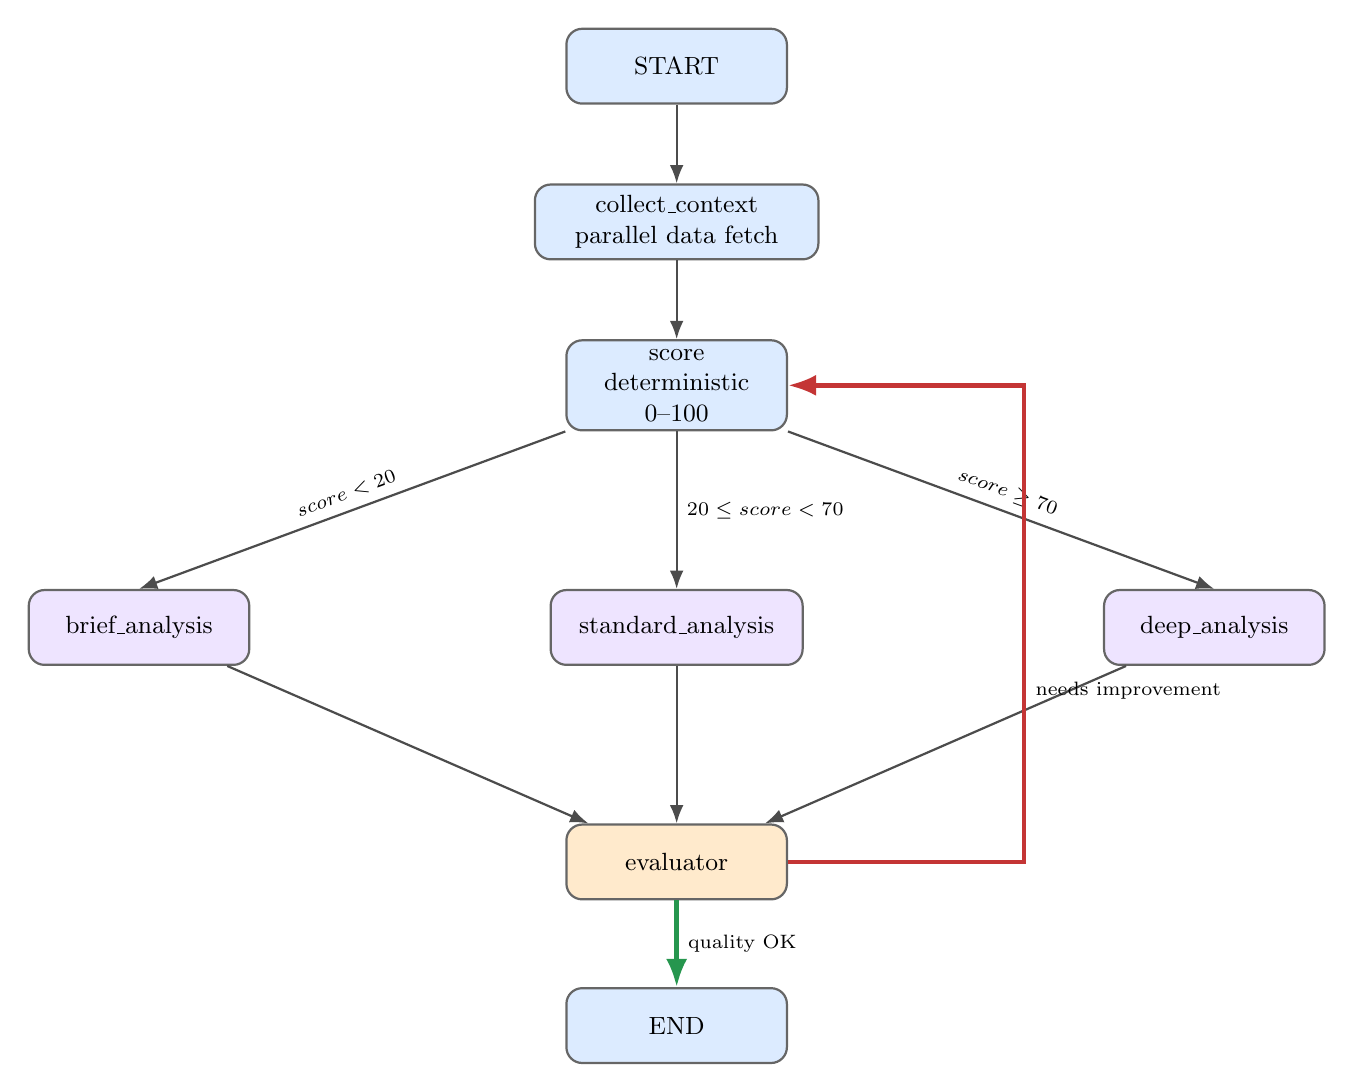
\begin{tikzpicture}[node distance=1.0cm and 1.6cm, font=\small]
    \node[datanode] (start2) {START};
    \node[datanode, below=1.0cm of start2, minimum width=3.6cm] (context) {collect\_context\\parallel data fetch};
    \node[datanode, below=1.0cm of context] (score) {score\\deterministic\\0--100};

    \node[llmnode, below left=2.0cm and 4.0cm of score] (brief) {brief\_analysis};
    \node[llmnode, below=2.0cm of score, minimum width=3.2cm] (standard) {standard\_analysis};
    \node[llmnode, below right=2.0cm and 4.0cm of score] (deep) {deep\_analysis};
    \node[evalnode, below=2.0cm of standard] (eval) {evaluator};
    \node[datanode, below=1.1cm of eval] (end2) {END};

    \draw[line] (start2) -- (context);
    \draw[line] (context) -- (score);
    \draw[line] (score.south west) -- node[above, sloped, font=\scriptsize] {$score < 20$} (brief.north);
    \draw[line] (score) -- node[right, font=\scriptsize] {$20 \leq score < 70$} (standard);
    \draw[line] (score.south east) -- node[above, sloped, font=\scriptsize] {$score \geq 70$} (deep.north);
    \draw[line] (brief) -- (eval);
    \draw[line] (standard) -- (eval);
    \draw[line] (deep) -- (eval);
    \draw[successline] (eval) -- node[right, font=\scriptsize, black] {quality OK} (end2);
    \draw[retryline] (eval.east) -- ++(3.0,0) |- node[pos=0.18, right, font=\scriptsize, black] {needs improvement} (score.east);
\end{tikzpicture}
\caption{Building Risk Graph topology. Blue boxes are deterministic/data nodes, purple boxes are LLM analysis nodes, the orange box is the evaluator, the green arrow is the success path, and the red arrow is the retry loop.}
\label{fig:building-topology}
\end{figure}

\subsection{State Definition}

\begin{lstlisting}[style=codestyle, language=Python]
class BuildingRiskState(TypedDict, total=False):
    building: dict[str, Any]         # user-submitted form data
    location: dict[str, Any] | None  # GPS coordinates
    context: dict[str, Any]          # fetched fault/seismic data
    componentScores: dict[str, int]  # per-component scores
    totalScore: int                  # 0-100 aggregate
    level: RiskLevel                 # dusuk/orta/yuksek/kritik
    summary: str                     # LLM-generated narrative
    recommendedActions: list[str]
    evaluator_feedback: str | None   # injected on retry
    retry_count: int
\end{lstlisting}

\subsection{Well-Defined Steps (Nodes)}

\begin{table}[H]
\centering
\begin{tabular}{@{}lll@{}}
\toprule
\textbf{Node} & \textbf{Type} & \textbf{Responsibility} \\
\midrule
\texttt{collect\_context}    & I/O (parallel)   & Fetch fault lines, historical \& recent quakes \\
\texttt{score}               & Deterministic    & Rule-based scoring across 5 components \\
\texttt{brief\_analysis}     & LLM (structured) & 2-3 sentence summary for low-risk buildings \\
\texttt{standard\_analysis}  & LLM (structured) & 2-paragraph analysis for medium risk \\
\texttt{deep\_analysis}      & LLM (structured) & 3-paragraph detailed analysis for high/critical \\
\texttt{evaluator}           & LLM (structured) & Judge quality; inject feedback or approve \\
\bottomrule
\end{tabular}
\caption{Building Risk Graph nodes and their single responsibilities.}
\end{table}

\subsection{Parallel Context Collection}

The \texttt{collect\_context} node uses \texttt{asyncio.gather} to fetch three data sources simultaneously, minimising latency:

\begin{lstlisting}[style=codestyle, language=Python]
fault_geojson, hist_events, recent_events = await asyncio.gather(
    client.fault_lines(bbox=bbox, simplify=0.008),
    client.historical_events(years=100, min_magnitude=4.5),
    client.recent_earthquakes(hours=168, min_magnitude=3.0, limit=120),
)
\end{lstlisting}

The node then computes the nearest active fault using a point-to-segment Haversine algorithm and extracts seismic gap signals (years since last M6+ event on the same fault corridor).

\subsection{Deterministic Score Engine}

The \texttt{score} node uses no LLM. It computes five components with fixed rules:

\begin{table}[H]
\centering
\begin{tabular}{@{}llr@{}}
\toprule
\textbf{Component} & \textbf{Key Factors} & \textbf{Max Score} \\
\midrule
Structural         & Construction year, floors, system, retrofit    & 35 \\
Soil               & Zone class ZA--ZF                              & 15 \\
Fault Proximity    & Distance, slip rate (mm/yr), seismic gap       & 20 \\
Historical Seismicity & Nearby M4.5+ count, max magnitude           & 15 \\
Observed Damage    & Column cracks, past damage                     & 20 \\
\midrule
\textbf{Total}     &                                                & \textbf{100} \\
\bottomrule
\end{tabular}
\caption{Scoring components in the deterministic rule engine.}
\end{table}

\begin{lstlisting}[style=codestyle, language=Python]
def _risk_level(total: int) -> tuple[RiskLevel, str]:
    if total < 20:  return "dusuk",  "Dusuk risk"
    if total < 45:  return "orta",   "Orta risk"
    if total < 70:  return "yuksek", "Yuksek risk"
    return "kritik", "Kritik risk"
\end{lstlisting}

\subsection{Score-Based Conditional Routing}

After scoring, a conditional edge selects the analysis depth:

\begin{lstlisting}[style=codestyle, language=Python]
def _route_by_score(state: BuildingRiskState) -> str:
    total = state.get("totalScore", 0)
    if total < 20:   return "brief_analysis"
    if total < 70:   return "standard_analysis"
    return "deep_analysis"

g.add_conditional_edges("score", _route_by_score, {
    "brief_analysis":    "brief_analysis",
    "standard_analysis": "standard_analysis",
    "deep_analysis":     "deep_analysis",
})
\end{lstlisting}

\subsection{Agentic Evaluator Loop}

All three analysis nodes feed into \texttt{evaluator}. This node uses a \textbf{second LLM call} to judge the generated summary against four quality criteria. If the quality is insufficient and the retry budget remains, it injects feedback into the state and routes back to \texttt{score}, re-entering the full analysis pipeline:

\begin{lstlisting}[style=codestyle, language=Python]
async def evaluator_node(state: BuildingRiskState) -> BuildingRiskState:
    # Fast structural checks before calling LLM (saves tokens)
    min_words = {"dusuk": 15, "orta": 25, "yuksek": 35, "kritik": 35}
    if len(summary.split()) < min_words.get(level, 20):
        return {
            "evaluator_feedback": "Ozet cok kisa. Daha ayrintili yaz.",
            "retry_count": retry_count + 1,
        }

    # Full LLM evaluation
    llm = get_structured_llm(EvaluatorOutput)
    result: EvaluatorOutput = await llm.ainvoke([...])

    if result.quality_ok:
        return {"evaluator_feedback": None}         # approve -> END

    return {
        "evaluator_feedback": result.feedback,      # inject feedback
        "retry_count": retry_count + 1,             # retry -> score
    }

def _route_evaluator(state: BuildingRiskState) -> str:
    if state.get("evaluator_feedback") and state.get("retry_count", 0) < MAX_RETRIES:
        return "score"    # re-enter pipeline with feedback
    return END
\end{lstlisting}

\begin{designnote}
The key insight is that graph state does more than store data: it also carries corrective feedback between nodes. When the evaluator rejects a weak answer, its feedback is written into \texttt{evaluator\_feedback}, and the next analysis attempt reads that field and revises the prompt. This creates a built-in self-correcting loop without any external orchestration code.
\end{designnote}

% ============================================================
\section{LangSmith Integration}
% ============================================================

\subsection{Configuration}

LangSmith tracing is fully configured and active. Three environment variables are set in \texttt{graph/.env}:

\begin{lstlisting}[style=codestyle]
LANGCHAIN_TRACING_V2=true
LANGCHAIN_PROJECT=seismic-command
LANGCHAIN_API_KEY=lsv2_pt_...
\end{lstlisting}

The \texttt{config.py} module reads these at startup:

\begin{lstlisting}[style=codestyle, language=Python]
LANGSMITH_TRACING = os.environ.get("LANGCHAIN_TRACING_V2", "false").lower() == "true"
LANGSMITH_PROJECT = os.environ.get("LANGCHAIN_PROJECT", "seismic-command")
\end{lstlisting}

\subsection{What LangSmith Traces}

Because LangGraph natively integrates with LangSmith, every run automatically records:

\begin{itemize}[leftmargin=1.5em]
    \item The full graph execution trace with each node's input and output
    \item Every LLM call with prompt, response, latency, and token count
    \item The evaluator feedback loop iterations (visible as nested spans)
    \item Classification decisions (keyword vs.\ LLM path)
\end{itemize}

\begin{figure}[H]
    \centering
    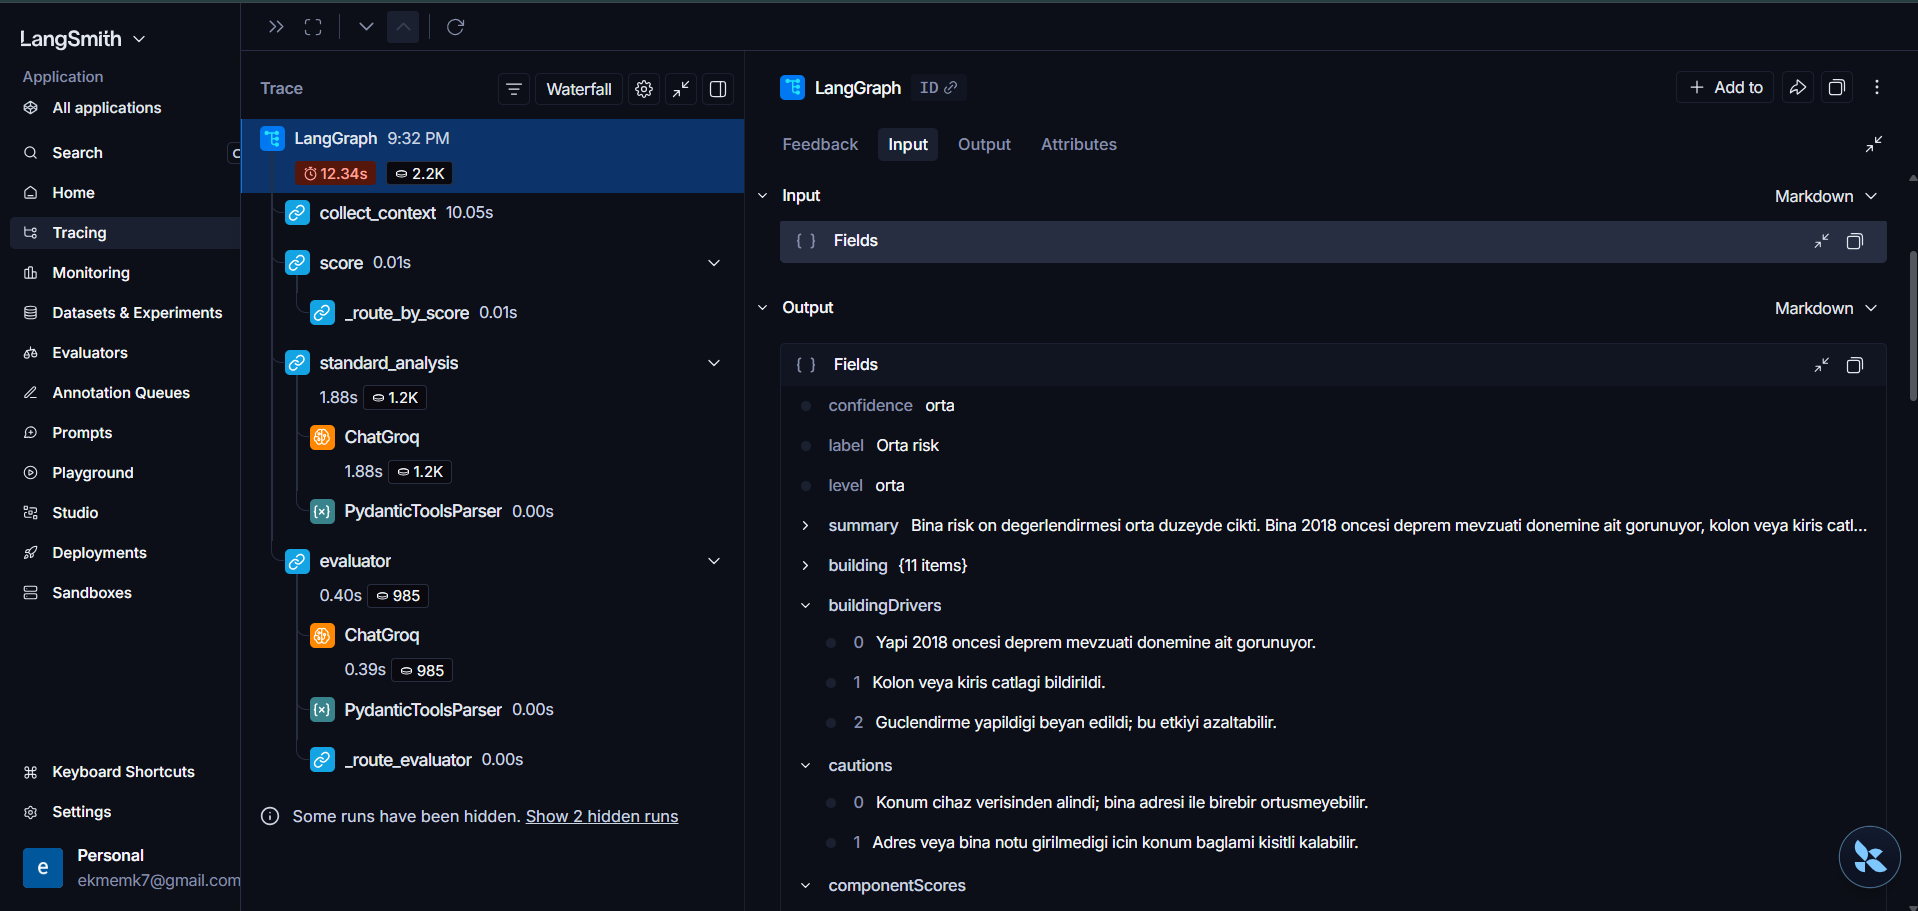
\includegraphics[width=\textwidth]{8.png}
    \caption{LangSmith trace view for a single Building Risk Graph run. The left panel shows the execution path through \texttt{collect\_context}, \texttt{score}, \texttt{\_route\_by\_score}, \texttt{standard\_analysis}, and \texttt{evaluator}. The right panel exposes the structured result returned by the graph, including the risk label, confidence value, summary, driver lists, warnings, and component scores. This screenshot demonstrates that each node in the workflow can be inspected individually, which makes the graph both debuggable and explainable.}
    \label{fig:langsmith}
\end{figure}

\begin{figure}[H]
    \centering
    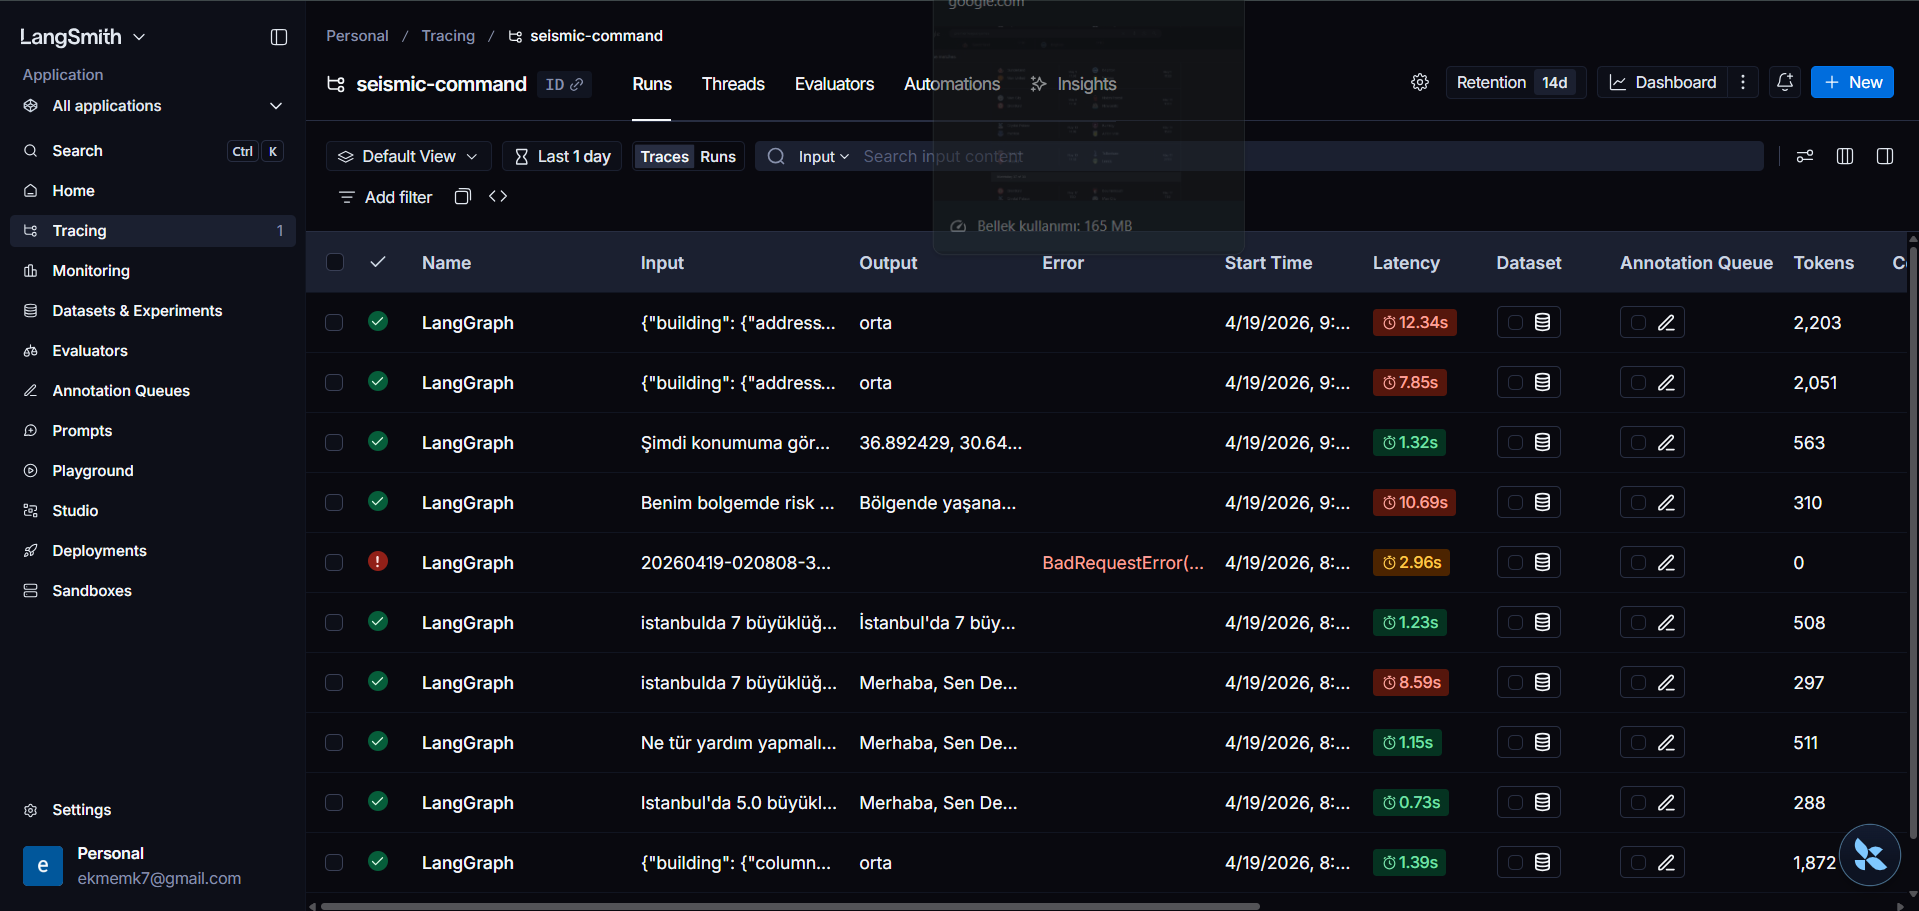
\includegraphics[width=\textwidth]{9.png}
    \caption{LangSmith project-level run list for the \texttt{seismic-command} project. This interface shows that both chat runs and building-risk runs are traced under the same project, together with timestamps, latency, token usage, and error status. In the report, this screenshot serves as evidence that LangSmith integration is active during real application usage rather than isolated development tests.}
    \label{fig:langsmith-runlist}
\end{figure}

\subsection{Why LangSmith Matters}

\begin{rationale}
Without LangSmith, debugging the evaluator retry loop requires reading log files and manually correlating LLM calls. With LangSmith, each retry appears as a nested span showing exactly which feedback was injected, which analysis node re-ran, and whether the second attempt passed evaluation. This visibility is essential during development and demonstrates that the agentic loop is functioning as designed.
\end{rationale}

% ============================================================
\section{CrewAI and LangGraph Coexistence}
% ============================================================

The assignment explicitly requires that LangGraph be added to an \textbf{existing project alongside CrewAI}, with both working simultaneously. This is achieved through service isolation:

\begin{itemize}[leftmargin=1.5em]
    \item \textbf{CrewAI} remains available as its own Python service on port \texttt{8001}, focused on multi-agent research and report generation.
    \item \textbf{LangGraph} runs as a separate FastAPI service on port \texttt{8002}, focused on stateful chat and agentic building-risk evaluation.
    \item \textbf{Spring Boot} stays in the middle and proxies both AI layers through its existing REST surface, so the Angular frontend can keep using one backend entry point.
    \item The two frameworks therefore coexist in the same repository and product without runtime conflict: different services, different endpoints, shared application domain.
\end{itemize}

\begin{successbox}{Integration Status}
Both frameworks are active in the same project. LangGraph endpoints are started with \texttt{uvicorn seismic\_graph.api:app --port 8002}, CrewAI is started from its own service on port \texttt{8001}, and the Angular frontend reaches both through the Spring Boot proxy layer.
\end{successbox}

% ============================================================
\section{API Endpoints}
% ============================================================

\begin{table}[H]
\centering
\begin{tabular}{@{}lll@{}}
\toprule
\textbf{Endpoint} & \textbf{Graph} & \textbf{Description} \\
\midrule
\texttt{POST /graph/chat}           & Chat Graph          & Multi-turn stateful chat \\
\texttt{GET  /graph/chat/stream}    & Chat Graph          & SSE token streaming \\
\texttt{POST /graph/building-risk}  & Building Risk Graph & Agentic risk assessment \\
\texttt{GET  /health}               & ---                 & Service health check \\
\bottomrule
\end{tabular}
\caption{FastAPI endpoints that form the main LangGraph submission scope.}
\end{table}

\begin{designnote}
These endpoints are enough to demonstrate the assignment requirements: clearly defined graph steps, conditional routing, persistent state, and an evaluator loop. They are also the two flows already connected to visible frontend screens, which makes the implementation easy to demo live.
\end{designnote}

% ============================================================
\section{Screenshots}
% ============================================================

\begin{figure}[H]
    \centering
    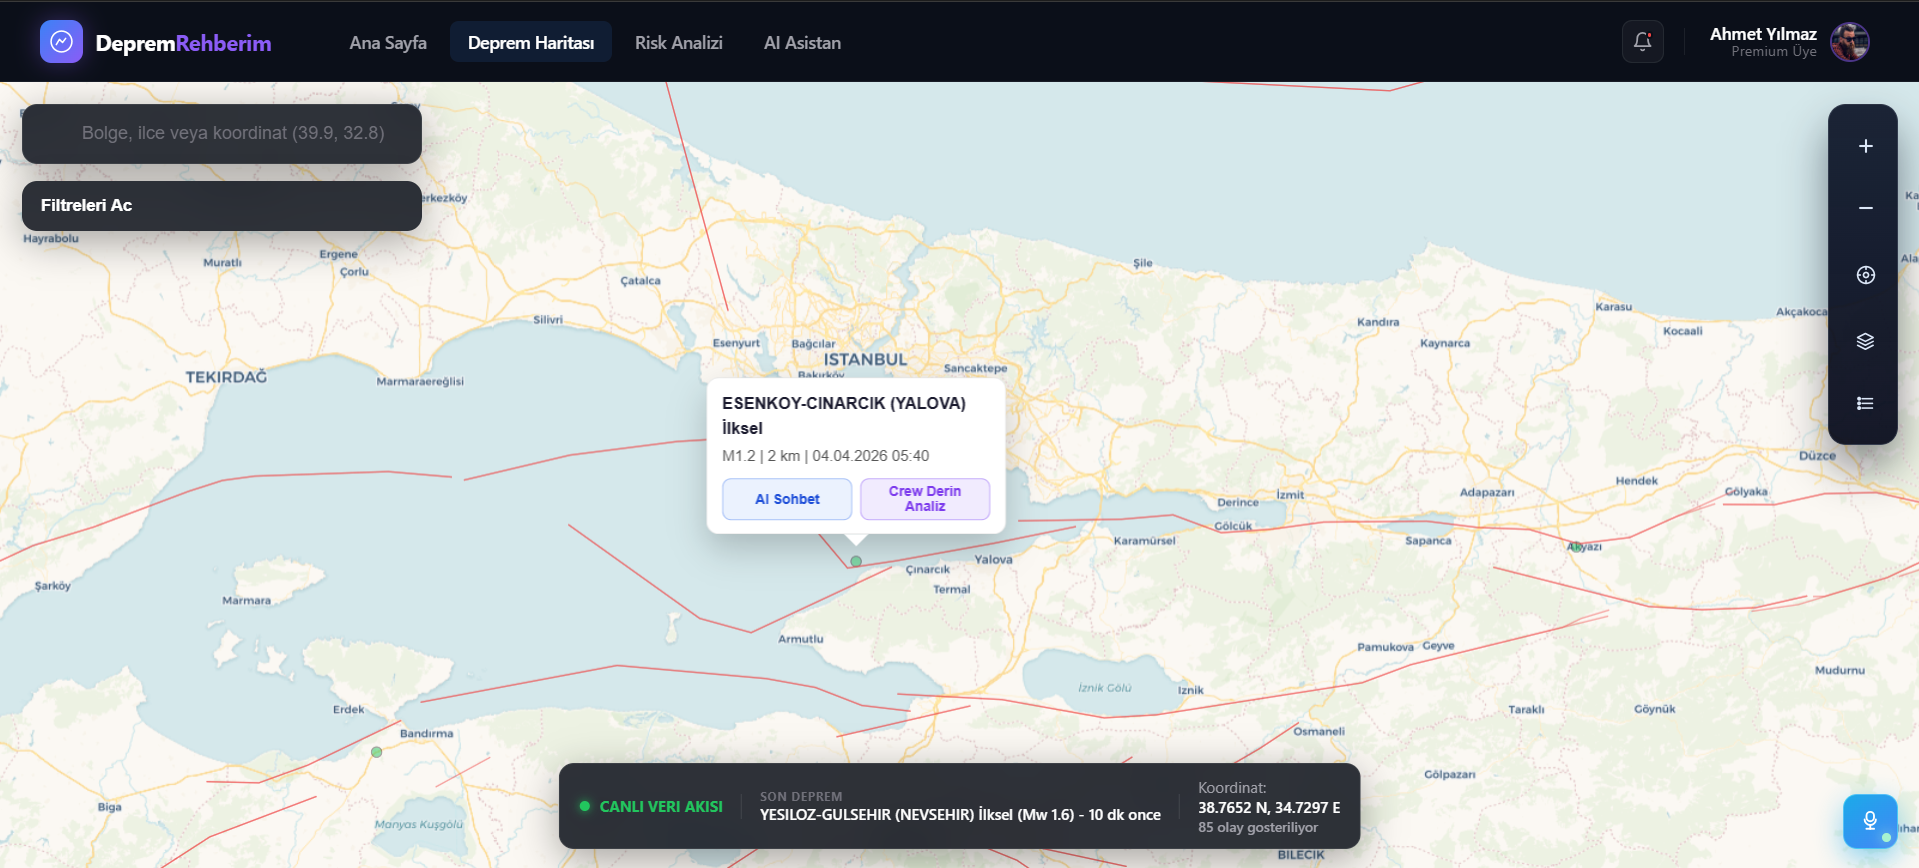
\includegraphics[width=\textwidth]{1.png}
    \caption{AI Assistant without location permission. The user asks a location-dependent risk question, and the Chat Graph routes the request to the \texttt{risk\_no\_loc} branch because the system does not yet have the user's coordinates. Instead of generating a potentially misleading region-specific answer, the assistant explicitly asks for location context. This screenshot demonstrates conditional routing based on missing state.}
    \label{fig:chat-no-location}
\end{figure}

\begin{figure}[H]
    \centering
    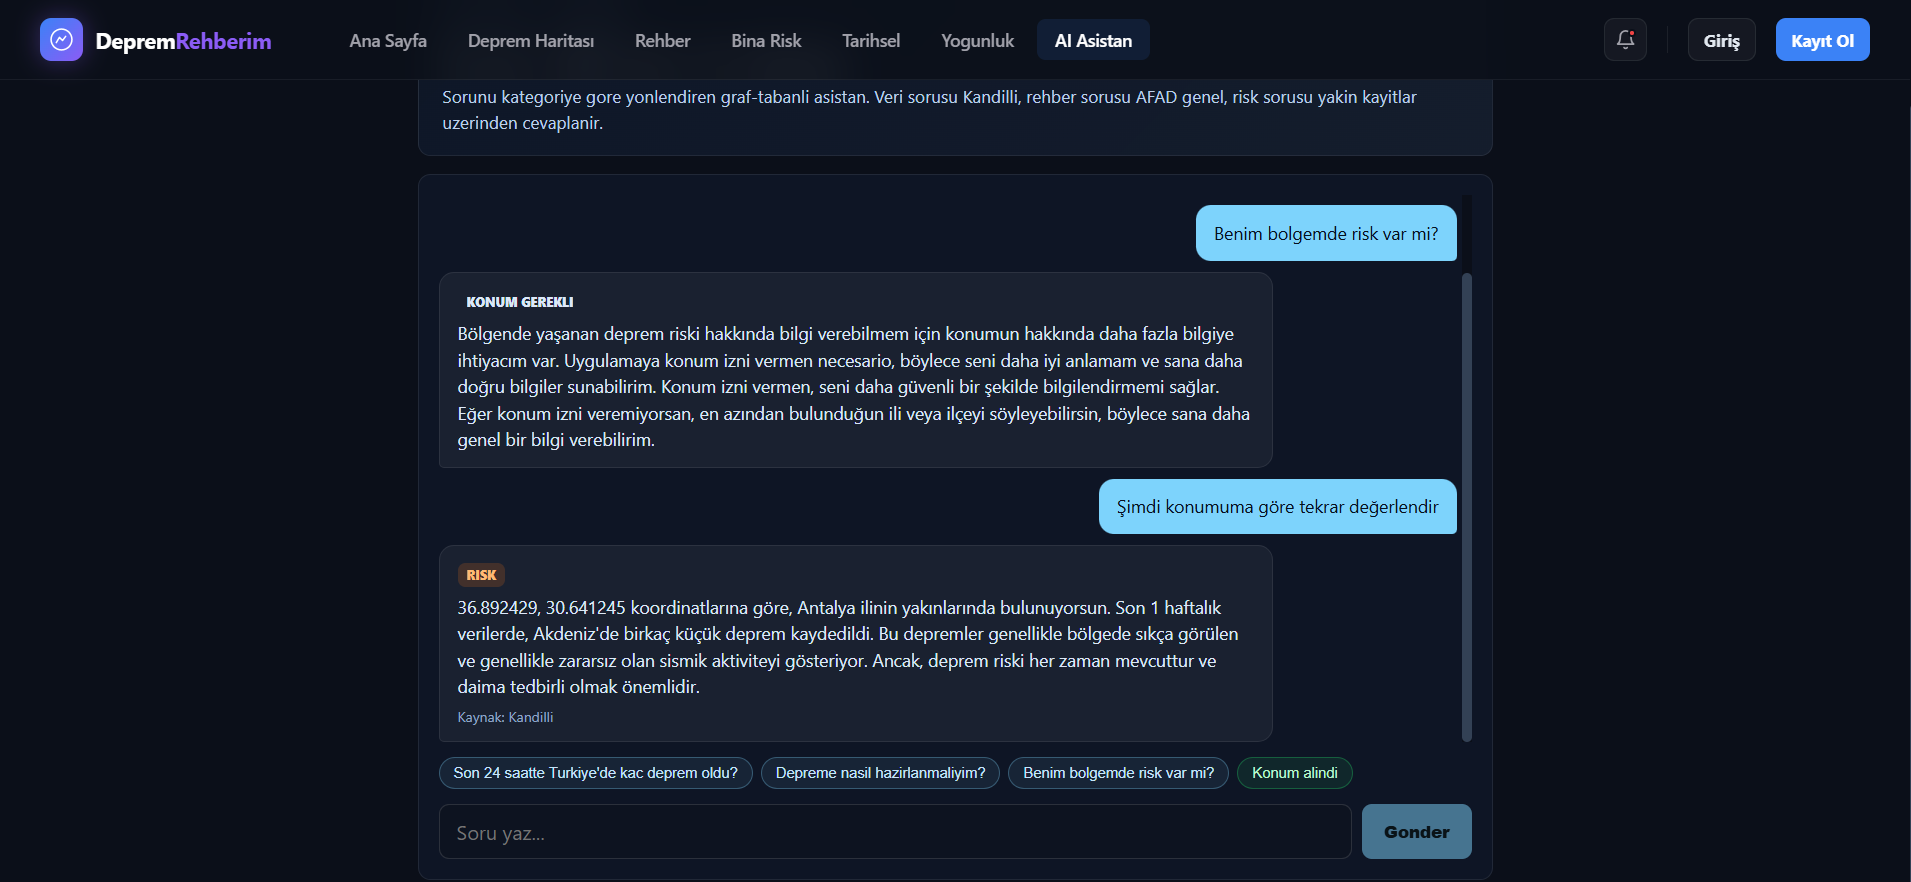
\includegraphics[width=\textwidth]{2.png}
    \caption{AI Assistant after location sharing in the same session. The earlier \texttt{risk\_no\_loc} response remains visible in the conversation history, and the follow-up request is now answered through the normal risk-analysis path using the newly available coordinates. The screenshot demonstrates multi-turn state persistence, category re-routing, and source attribution in a single conversational flow.}
    \label{fig:chat-with-location}
\end{figure}

\begin{figure}[H]
    \centering
    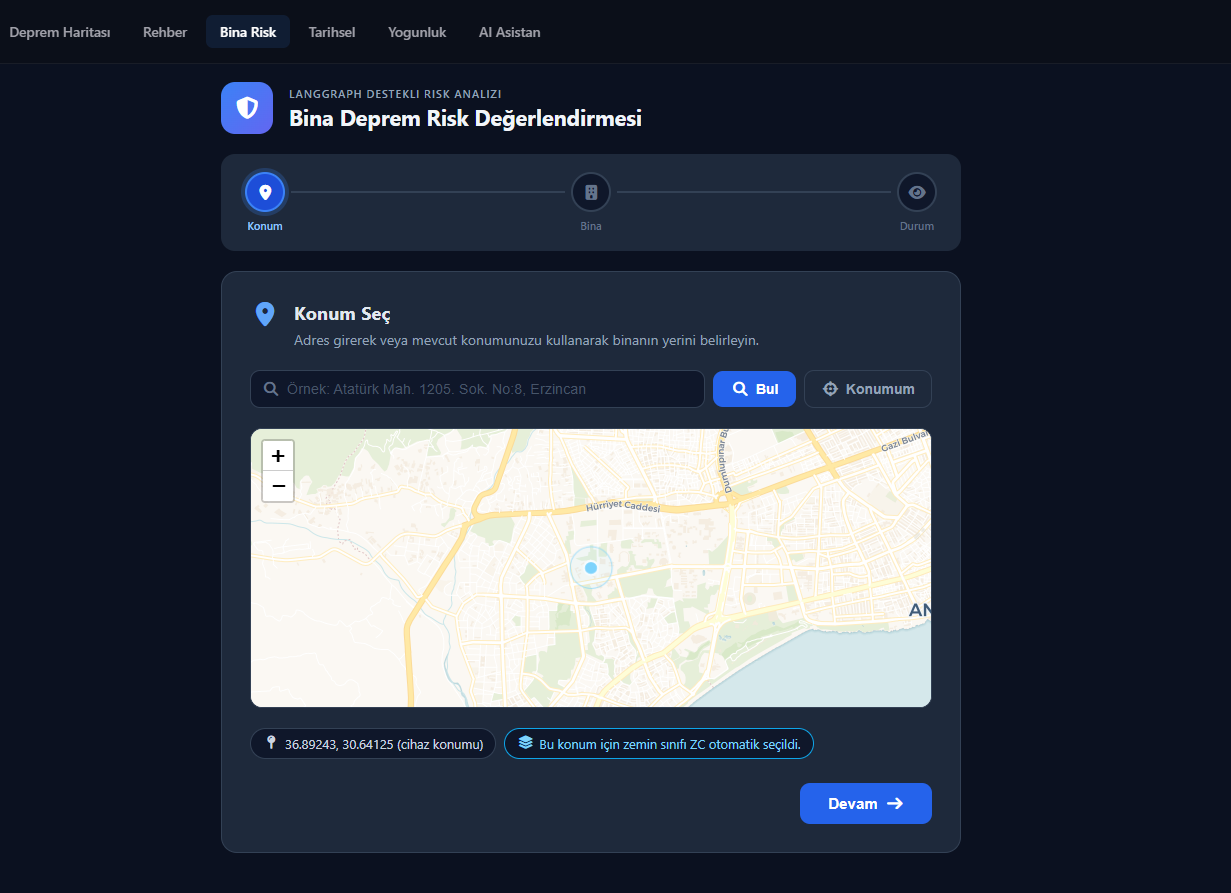
\includegraphics[width=0.82\textwidth]{3.png}
    \caption{Building Risk workflow, step 1: location selection. The user chooses the building location on the map, and the application automatically derives contextual data such as approximate coordinates and the soil class at that point. This visual matters because the graph uses not only typed building attributes, but also geospatial context gathered before scoring begins.}
    \label{fig:building-location}
\end{figure}

\begin{figure}[H]
    \centering
    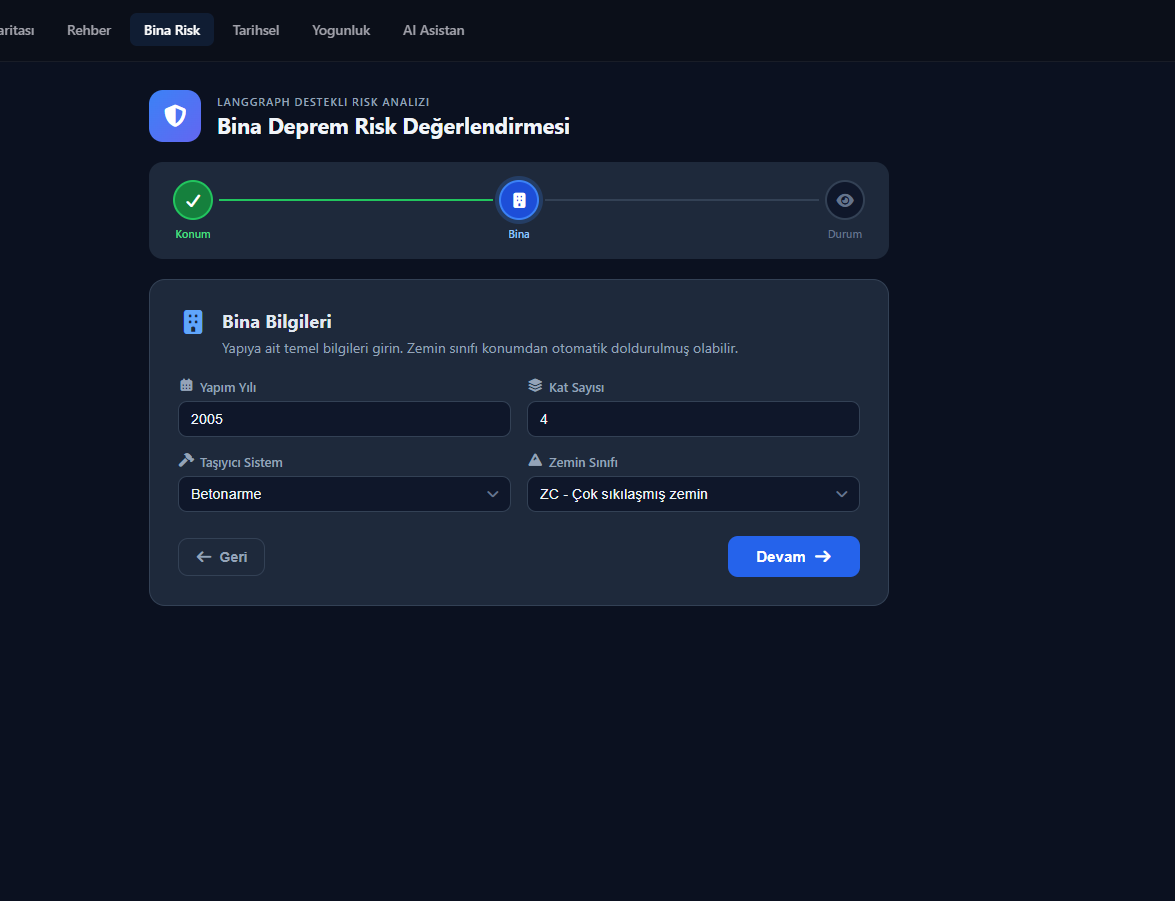
\includegraphics[width=0.82\textwidth]{4.png}
    \caption{Building Risk workflow, step 2: structural data entry. The user provides the construction year, floor count, structural system, and soil type of the building. These values form the deterministic input for the structural and soil components of the risk score, so this screenshot documents the frontend-to-graph data contract for the main assessment workflow.}
    \label{fig:building-form}
\end{figure}

\begin{figure}[H]
    \centering
    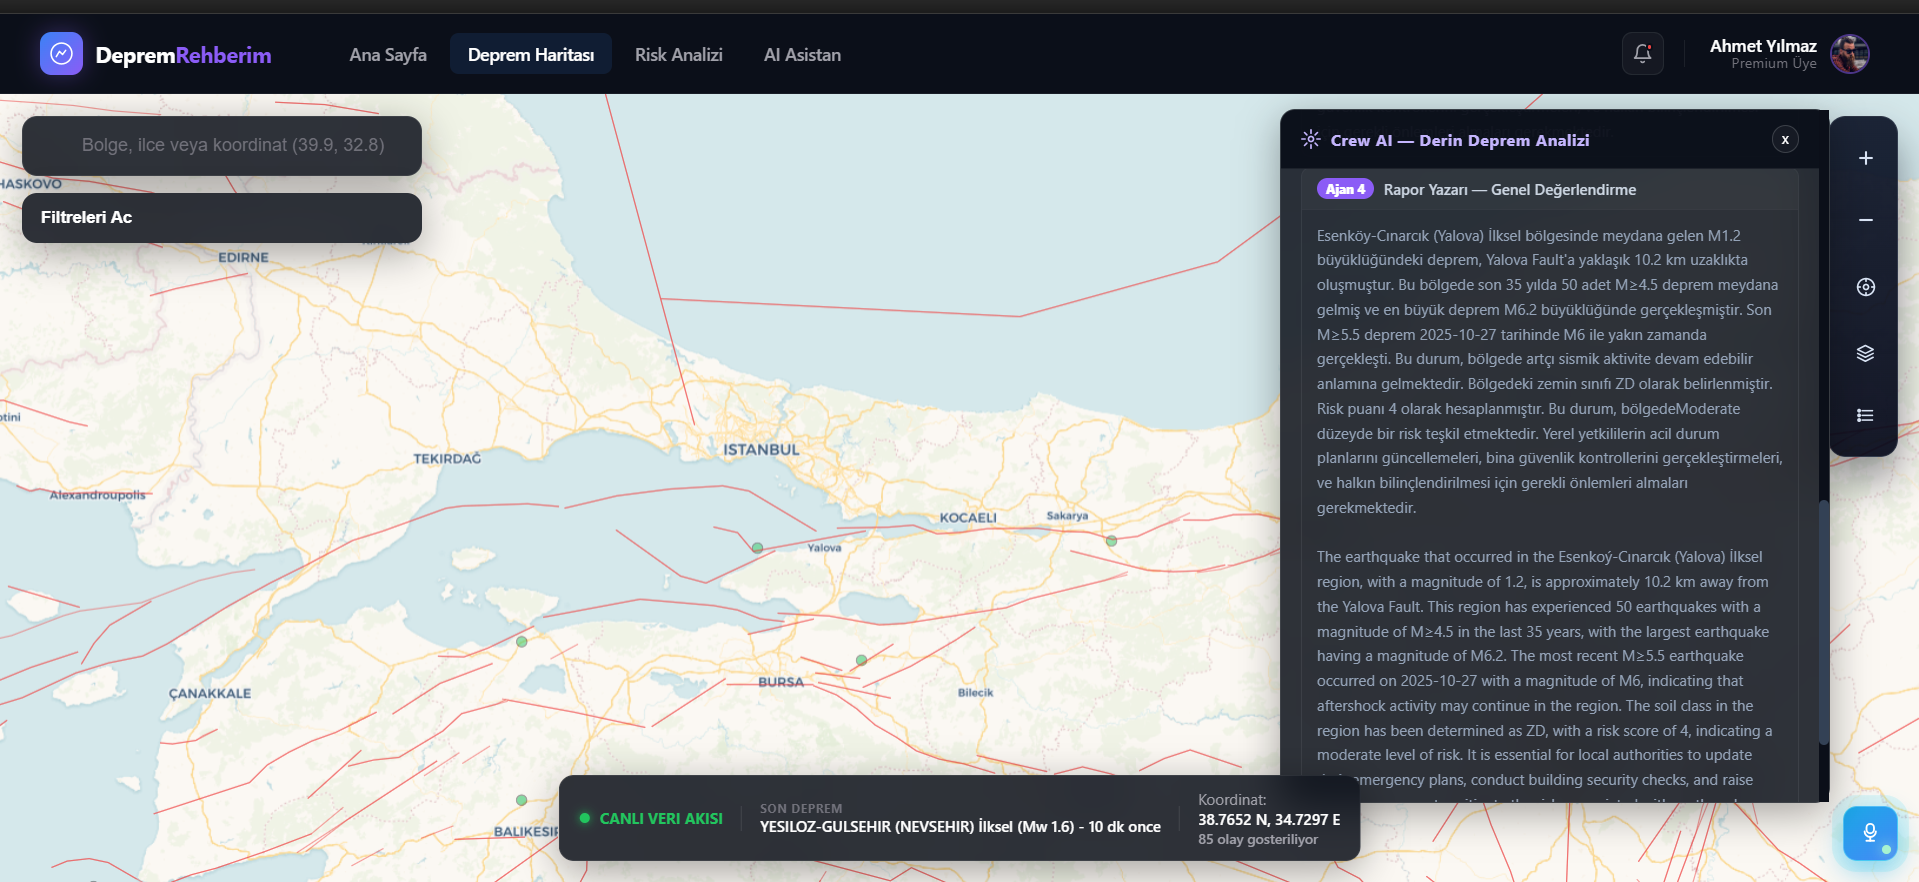
\includegraphics[width=0.82\textwidth]{5.png}
    \caption{Building Risk workflow, step 3: observed-condition selection. The user marks visible conditions such as cracks, soft-storey risk, past damage, irregularity, and retrofit status. Inside the graph, these selections are translated into deterministic score contributions before the natural-language explanation is generated. This screenshot shows that the final result is grounded in explicit evidence rather than unconstrained prompting alone.}
    \label{fig:building-observed}
\end{figure}

\begin{figure}[H]
    \centering
    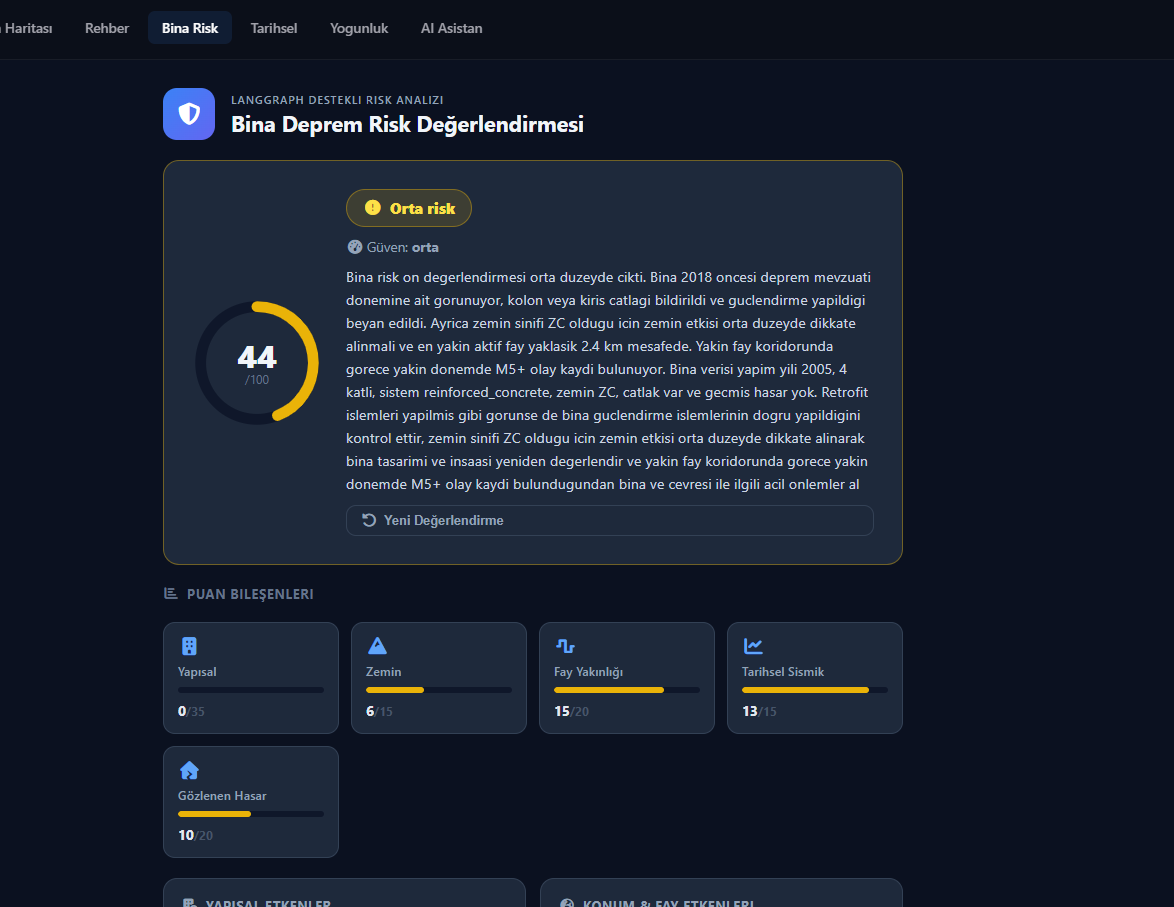
\includegraphics[width=0.82\textwidth]{6.png}
    \caption{Building Risk result overview. After graph execution, the interface presents the total score, the interpreted risk level, a confidence indicator, and a Turkish summary that combines deterministic scoring with LLM-based explanation. This screenshot is one of the strongest pieces of evidence in the report because it shows the transformation from structured inputs into a user-facing decision output.}
    \label{fig:building-result-overview}
\end{figure}

\begin{figure}[H]
    \centering
    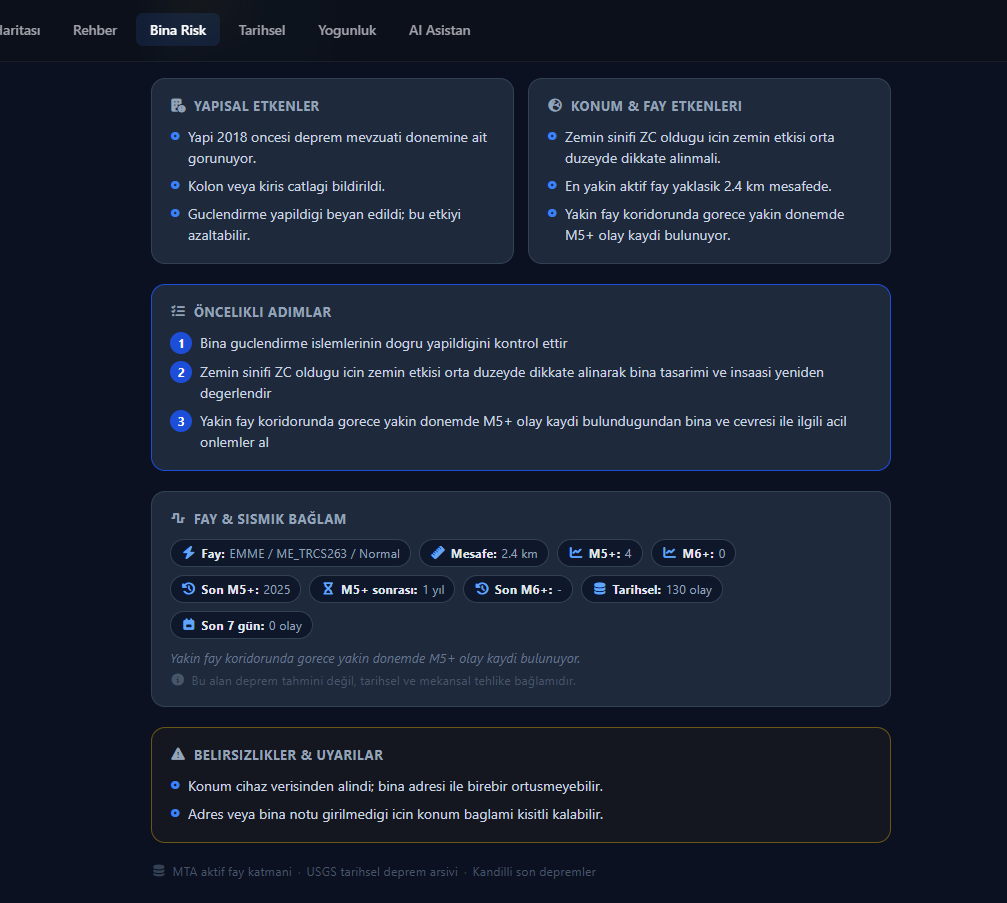
\includegraphics[width=0.82\textwidth]{7.png}
    \caption{Building Risk result details. Beyond the headline score, the interface exposes structural drivers, location and fault-related drivers, recommended priority actions, fault-corridor metadata, historical seismic context, and uncertainty notes returned by the graph. This detailed screen is valuable because it shows that the system outputs not only a label such as ``medium risk,'' but also interpretable supporting evidence and actionable recommendations.}
    \label{fig:building-result-details}
\end{figure}


% ============================================================
\section{Reflection and Conclusion}
% ============================================================

\begin{reflectionbox}
\textbf{Graph topology makes intent explicit.} Expressing the logic as a directed graph with named nodes and conditional edges---rather than nested if-else blocks---makes the system's decision flow immediately readable. Adding a new question category to the Chat Graph is a matter of adding one node and one edge entry, not refactoring a function.
\end{reflectionbox}

\vspace{0.3em}

\begin{reflectionbox}
\textbf{Separating scoring from analysis was the right call.} The deterministic score engine in the Building Risk Graph has no LLM dependency, which means it runs in under 1ms, is fully testable, and is never affected by model randomness. The LLM layer only handles the parts that genuinely require language: generating the natural-language summary and evaluating its quality.
\end{reflectionbox}

\vspace{0.3em}

\begin{reflectionbox}
\textbf{The evaluator loop has real value.} In testing, the brief-analysis node occasionally produced summaries that were too short or omitted location factors. The evaluator catches these cases automatically and requests a more detailed retry. Without the loop, this quality check would have to be done manually or skipped entirely.
\end{reflectionbox}

\vspace{0.3em}

\begin{reflectionbox}
\textbf{LangSmith removes debugging guesswork.} The evaluator retry loop involves 3-4 LLM calls per request on a bad run. Without tracing, diagnosing why a summary was rejected requires adding print statements and re-running manually. LangSmith shows the full trace---including which feedback was injected and whether the second attempt passed---in a single browser tab.
\end{reflectionbox}

\vspace{0.5em}

In summary, LangGraph was integrated into the existing Seismic Command project to add stateful, graph-based AI orchestration alongside the pre-existing CrewAI agents. The two primary graphs---Chat and Building Risk---demonstrate the core LangGraph patterns required by the assignment: well-defined node steps, conditional routing, state management, and an agentic feedback loop, all observable through LangSmith tracing.

\end{document}
